\section{Social Network}\label{sec:fa_social_network}

The current design for the escolinhas.pt social network is dynamic in nature, and extracted from the relationships formed through the connections between users and their roles with schools, groups, and even another roles, as depicted in Fig.~\ref{fig:social_network_current}.

\begin{figure}[H]
  \centering
  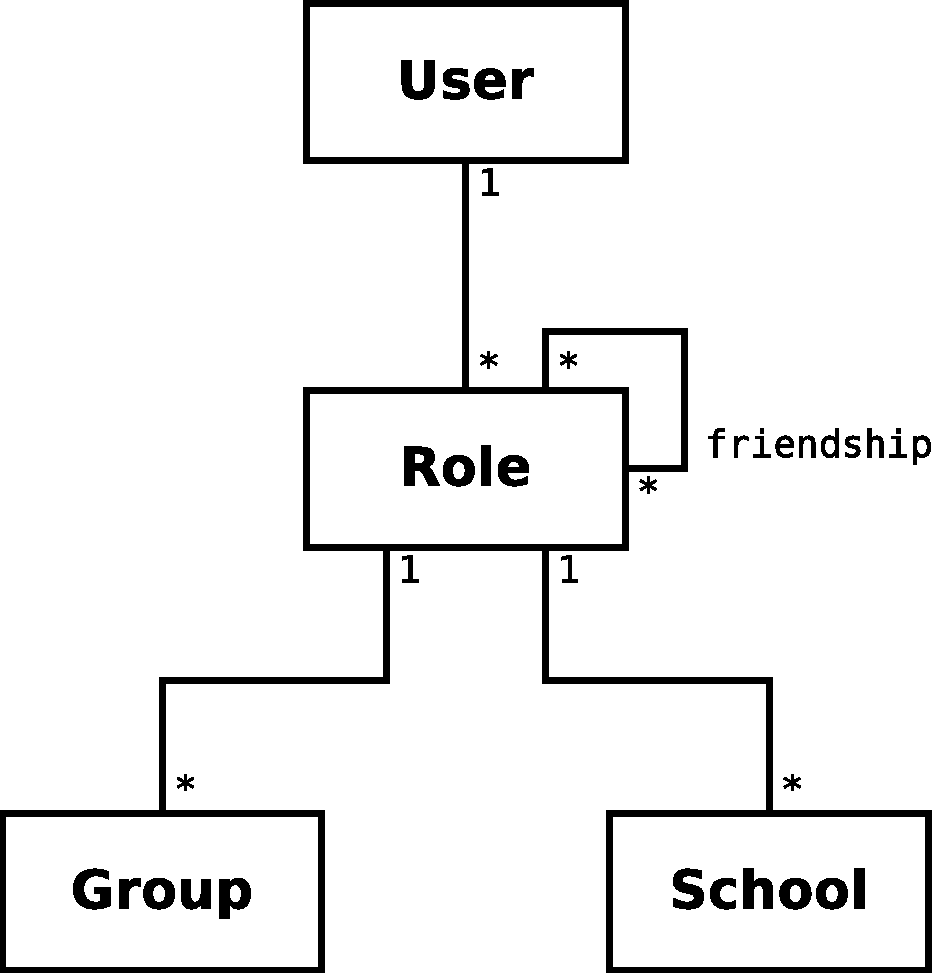
\includegraphics[width=65mm]{social_network_current.pdf}
  \caption{Current User Network Model}
  \label{fig:social_network_current}
\end{figure}

\subsection{Variability Requirements}\label{sec:fa_social_network_variability_requirements}

This model, however useful, offers a very small degree of variability. Due to the closed nature of the platform, there is a need to provide mechanisms able to fine-tune these connections in order to cater to each school specific needs. These mechanisms need to be available at the system administrator level, in order to easily manipulate these links without the need to pollute the application's codebase with hard-coded rules and without the need for redeployement.

\subsection{Candidate Patterns}\label{sec:fa_social_network_candidate_patterns}

Ideally, the user network would be described with a simple, self-referencing model, as shown in figure~\ref{fig:ideal_social_network_users}. This allows to create static relationships between any two users that can be edited as needed.

\begin{figure}[H]
  \centering
  %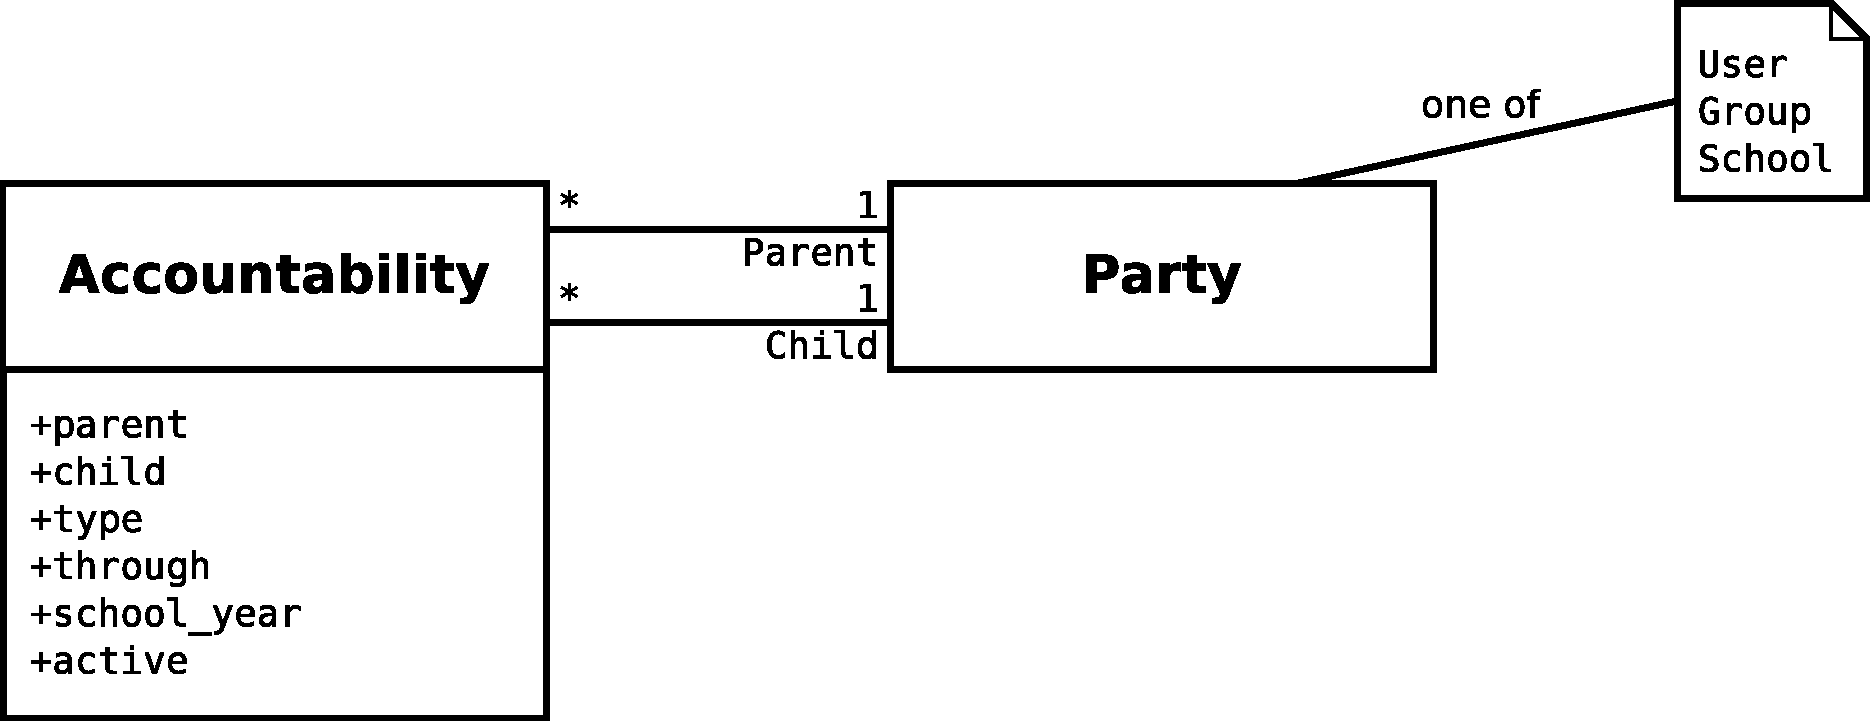
\includegraphics[width=65mm]{social_network_conceptual.pdf}
  \caption{Conceptual User Network Model}
  \label{fig:social_network_conceptual}
\end{figure}

\subsection{Chosen Patterns \& Rationale}\label{sec:fa_social_network_chosen_patterns_rationale}

A variant of the \textsc{Accountability} design pattern was chosen (shown in Fig.~\ref{fig:social_network_conceptual}). This implementation follows the original description of the pattern by using all the usual entities present in the original \textsc{Accountability} pattern \cite{fowler_accountability} - however, it denormalizes the AccountabilityType entity \emph{into} the Accountabilities themselves. Despite creating some data redundancy, this option provides a more performant implementation: as the Accountabilities table is to be constantly accessed, the decision to have the AccountabilityTypes in a separate table would lead to expensive \verb!JOIN! operations. This, in turn, would lead to a less than desirable performance and complexity. \textbf{I PROBABLY NEED TO BACK THIS UP WITH SOME DATA!!! ALSO THIS IS PROBABLY BETTER IF PLACED IN \ref{sec:fa_social_network_implementation}}

\begin{figure}[H]
  \centering
  %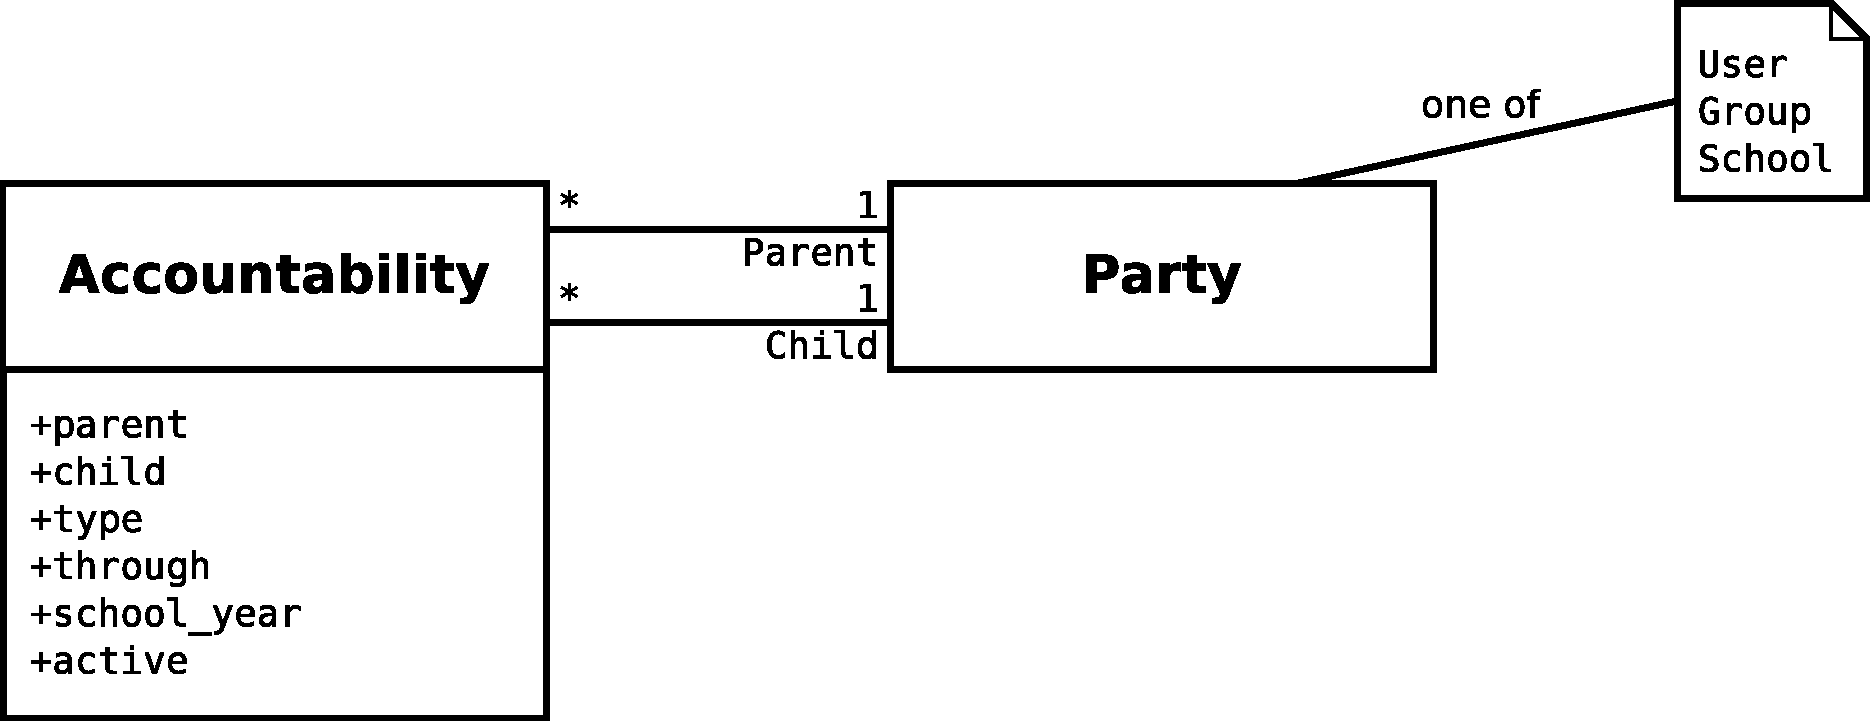
\includegraphics[width=65mm]{social_network_conceptual.pdf}
  \caption{Conceptual User Network Model}
  \label{fig:social_network_conceptual}
\end{figure}

\subsection{Implementation}\label{sec:fa_social_network_implementation}

\subsection{Impact Analysis}\label{sec:fa_social_network_impact_analysis}
